\documentclass{article}

% if you need to pass options to natbib, use, e.g.:
% \PassOptionsToPackage{numbers, compress}{natbib}
% before loading nips_2016
%
% to avoid loading the natbib package, add option nonatbib:
% \usepackage[nonatbib]{nips_2016}

% \usepackage{nips_2016}

% to compile a camera-ready version, add the [final] option, e.g.:
\usepackage[final]{nips_2016}

\usepackage[utf8]{inputenc} % allow utf-8 input
\usepackage[T1]{fontenc}    % use 8-bit T1 fonts
\usepackage{hyperref}       % hyperlinks
\usepackage{url}            % simple URL typesetting
\usepackage{booktabs}       % professional-quality tables
\usepackage{amsfonts}       % blackboard math symbols
\usepackage{nicefrac}       % compact symbols for 1/2, etc.
\usepackage{microtype}      % microtypography
\usepackage{amssymb}
\usepackage{mathbbol}
\usepackage{graphicx}

\title{10-703 - Homework 2: Playing Atari With Deep Reinforcement Learning}

% The \author macro works with any number of authors. There are two
% commands used to separate the names and addresses of multiple
% authors: \And and \AND.
%
% Using \And between authors leaves it to LaTeX to determine where to
% break the lines. Using \AND forces a line break at that point. So,
% if LaTeX puts 3 of 4 authors names on the first line, and the last
% on the second line, try using \AND instead of \And before the third
% author name.

\author{
  Rogerio~Bonatti\ \\
  Robotics Institute\\
  Carnegie Mellon University\\
  Pittsburgh, PA 15213 \\
  \texttt{rbonatti@andrew.cmu.edu} \\
  %% examples of more authors
  \And
  Ratnesh~Madaan\ \\
  Robotics Institute\\
  Carnegie Mellon University\\
  Pittsburgh, PA 15213 \\
  \texttt{ratneshm@andrew.cmu.edu} \\
  \And
  Adithya~Murali\ \\
  Robotics Institute\\
  Carnegie Mellon University\\
  Pittsburgh, PA 15213 \\
  \texttt{amurali@andrew.cmu.edu} \\
  \And
  Alex~Spitzer\ \\
  Robotics Institute\\
  Carnegie Mellon University\\
  Pittsburgh, PA 15213 \\
  \texttt{aspitzer@andrew.cmu.edu} \\
  %% \AND
  %% Coauthor \\
  %% Affiliation \\
  %% Address \\
  %% \texttt{email} \\
  %% \And
  %% Coauthor \\
  %% Affiliation \\
  %% Address \\
  %% \texttt{email} \\
  %% \And
  %% Coauthor \\
  %% Affiliation \\
  %% Address \\
  %% \texttt{email} \\
}

\begin{document}
% \nipsfinalcopy is no longer used

\maketitle

\begin{abstract}
  In this assignment we implemented various types of algorithms for control, including LQR, iLQR, Behavior Cloning and REINFORCE. 
\end{abstract}

\section{LQR}
Here are our results for the LQR algorithm. 

\subsection{[5pts] Test your LQR implementation on the TwoLinkArm-v0 environment. Record the total reward and number of steps to reach the goal. Also plot $q$, $\dot{q}$, and your control inputs $u$}

pass

\subsection{[5pts] Test your LQR implementation on the TwoLinkArm-limited-torque-v0 environment. Record the total reward and the number of steps to reach the goal. Also plot $q$, $\dot{q}$, and your control inputs $u$. Additionally plot u clipped to the action space of this environment.}

pass

\subsection{[5pts] Compare the performance of your controller on each of these environments}

pass

\subsection{[5pts] Test your LQR implementation on the TwoLinkArm-v1 environment. Record the total reward and number of steps to reach the goal. Also plot $q$, $\dot{q}$, and your control inputs $u$}

pass

\subsection{[5pts] Test your LQR implementation on the TwoLinkArm-limited-torque-v1 environment. Record the total reward and the number of steps to reach the goal. Also plot $q$, $\dot{q}$, and your control inputs $u$. Additionally plot u clipped to the action space of this environment.}

pass

\subsection{[5pts] Compare the performance on these environments to the v0 versions.}

pass





\section{iLQR}
Here are our results for the iLQR algorithm. 

\subsection{[10pts] Test your iLQR implementation on the TwoLinkArm-v0 environment. Plot the total cost (intermediate cost + final cost) respect to iterations and record the total reward. Also plot $q$, $\dot{q}$, and your control inputs $u$.}

pass

\subsection{[10pts] Test your iLQR implementation on the TwoLinkArm-v1 environment. Plot the total cost (intermediate cost + final cost) respect to iterations and record the total reward. Also plot $q$, $\dot{q}$, and your control inputs $u$.}

pass

\subsection{[5pts] Discuss the comparison between iLQR and LQR algorithm, which one is better and why?}

pass

\subsection{[5pts EXTRA CREDIT] iLQR is not as fast as we want. Try to improve the convergence in any way you can figure out. Potential directions include changing cost function and use better optimization procedures.}

pass




\section{Behavior cloning}
Here are our results for the behavior cloning algorithm. 

\subsection{[10pts] Use each of your datasets to train a cloned behavior using the dataset as a supervised learning problem. Record the final loss and accuracy of your model after training for at least 50 epochs. Make sure you include any hyper parameters in your report}

pass

\subsection{[[10pts] Evaluate each of your cloned models on the CartPole-v0 model using the test cloned policy method. How does the amount of training data affect the cloned policy?}

pass

\subsection{[10pts] Evaluate each of your cloned models on the CartPole-v0 domain wrapped with the wrap cartpole function. Also evaluate the expert policy. How does your cloned behavior compare with respect to the expert policies and each other.}

pass



\section{REINFORCE}
Here are our results for the REINFORCE algorithm. 

\subsection{[10pts] Train REINFORCE on CartPole-v0 until convergence. Show your learning curves for the agent. In other words, every k episodes, freeze the current cloned policy and run 100 test episodes. Average the total reward and track the min and max reward. Plot the total reward on the y-axis with min/max values as error-bars vs the number of training episodes.}

pass

\subsection{[10pts] How does this policy compare to our provided expert and your cloned models?}

pass





Updates:

\begin{equation} \label{eq:updateQ}
  Q(s,a) := Q(s,a) + \alpha \left(r+\gamma \max_{a' \in A} Q(s',a') - Q(s,a)\right) 
\end{equation}

\begin{equation} \label{eq:updatew}
  w := w + \alpha \left(r+\gamma \max_{a' \in A} Q(s',a') - Q(s,a)\right) \nabla_w  Q_w(s,a)
\end{equation}

\textbf{Solution:}

We begin with Eq~\ref{eq:updatew}, substituting the derivative with respect to $w$, given that $Q(s,a)=w^T\phi(s,a)$:

\begin{equation} \label{eq:derivation_1}
  w := w + \alpha \left(r+\gamma \max_{a' \in A} Q(s',a') - Q(s,a)\right) \phi(s,a)
\end{equation}

Now we transpose both sides of the equation, and multiply both sides by $\phi(s,a)$:

\begin{equation} \label{eq:derivation_2}
  w^T\phi(s,a) := w^T\phi(s,a) + \alpha \left(r+\gamma \max_{a' \in A} Q(s',a') - Q(s,a)\right) \phi^T(s,a) \phi(s,a)
\end{equation}

Now we can again use the fact that $Q(s,a)=w^T\phi(s,a)$:

\begin{equation} \label{eq:derivation_3}
  Q(s,a) := Q(s,a) + \alpha \left(r+\gamma \max_{a' \in A} Q(s',a') - Q(s,a)\right) \phi^T(s,a) \phi(s,a)
\end{equation}

Lastly, since $\phi(s,a)_{s',a'} = \mathbb{1}[s'=s, a'=a]$, the norm of the dot product will equal to 1, resulting in:

\begin{equation} \label{eq:derivation_4}
  Q(s,a) := Q(s,a) + \alpha \left(r+\gamma \max_{a' \in A} Q(s',a') - Q(s,a)\right)
\end{equation}

And this we proved that Eq~\ref{eq:updatew} is the same as Eq~\ref{eq:updateQ}.

\section{[5pts] Implement a linear Q-network (no experience replay or target fixing). Use the experimental setup of \cite{mnih2013playing,mnih2015human} to the extent possible}

We implemented a linear Q-network, and to run the training process, one needs to run the command ``python dqn.py --modes ''.

We used the following hyper-parameters for this network:
\begin{itemize}
  \item Discount factor $\gamma=0.99$
  \item Learning rate $\alpha=0.0001$
  \item Exploration probability $\epsilon=0.05$, decreasing from $1$ to $0.05$ in a linear fashion during training process
  \item Number of iterations with environment: 5,000,000
  \item Number of frames to feed to the Q-network: 4
  \item Input image resizing: $84\times84$
  % \item Replay buffer size: 1,000,000
  % \item Target Q-network reset interval: 10,000
  % \item Batch size: 32
  \item Steps between evaluations of network: 10,000
  \item Steps for ``burn in'' (random actions in the beginning of training process): 50,000
  \item Maximum episode length: 100,000 steps (basically we chose to allow any game size)
\end{itemize}

We plotted the performance plots of this network in Figs~\ref{fig:q_q2}-\ref{fig:r_q2}.

\begin{figure}[ht] \label{fig:q_q2}
  \centering
  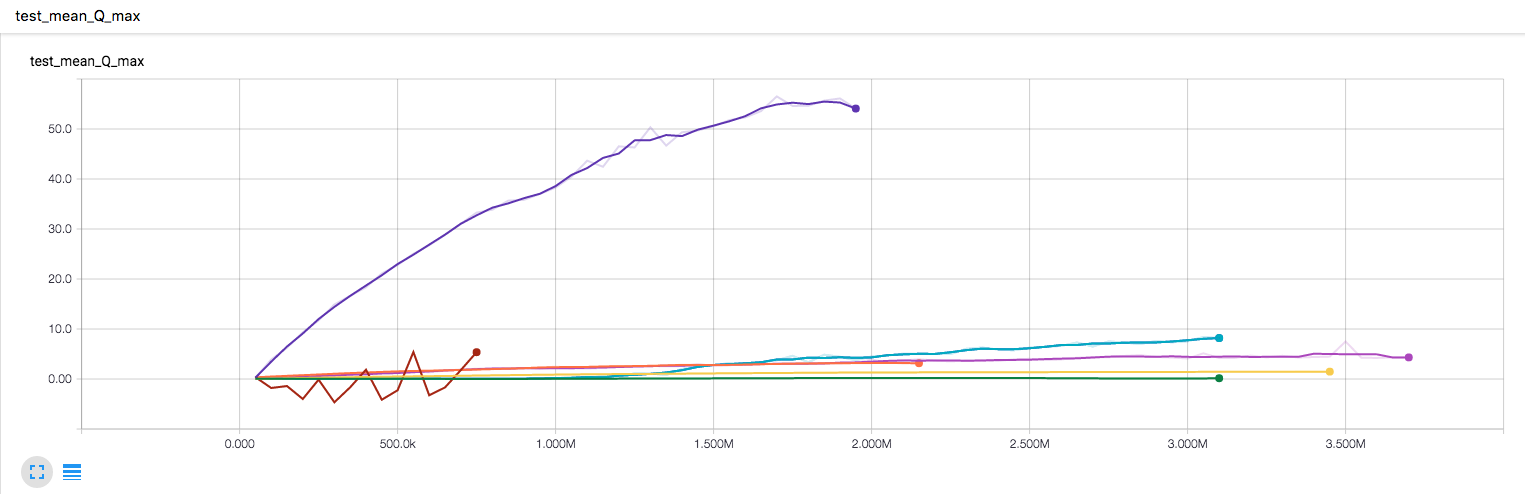
\includegraphics[width=1.0\textwidth]{images/q_linearWithoutStuff}
  \caption{Mean Q per step plot for the case of linear network without target fixing and without experience replay}
\end{figure}

\begin{figure}[ht] \label{fig:r_q2}
  \centering
  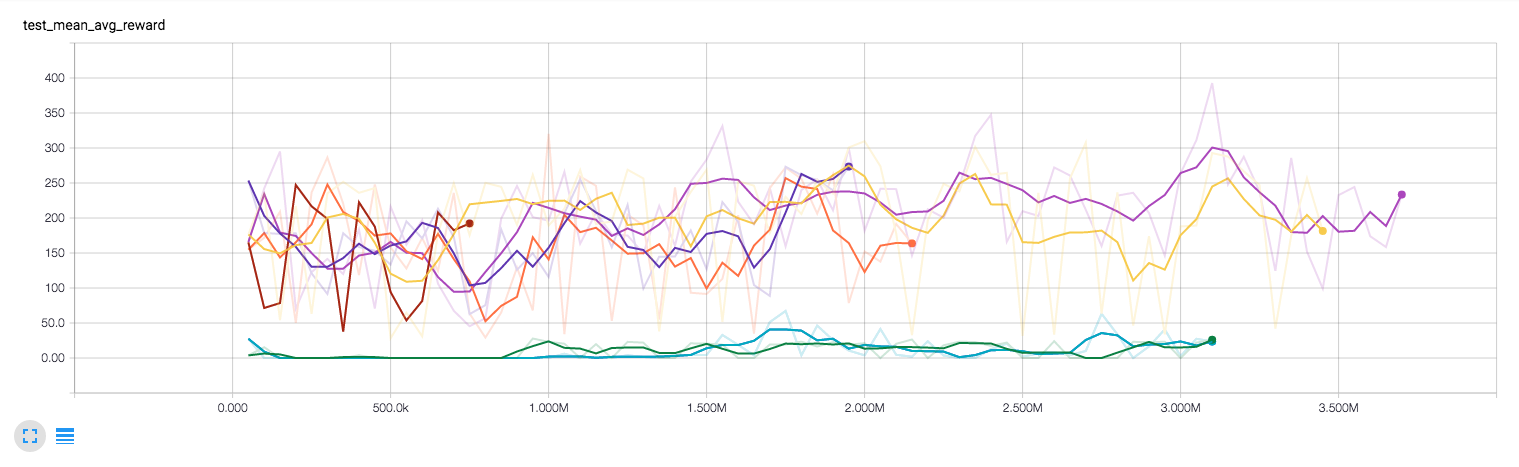
\includegraphics[width=1.0\textwidth]{images/r_linearWithoutStuff}
  \caption{Mean reward per episode plot for the case of linear network without target fixing and without experience replay}
\end{figure}

Using the \textit{Monitor} wrapper of the gym environment, we generated videos of the behavior of the agent across different stages of training:

\begin{itemize}
  \item 0/3 of training: \href{http://www.sharelatex.com}{Youtube video}
  \item 1/3 of training: \href{http://www.sharelatex.com}{Youtube video}
  \item 2/3 of training: \href{http://www.sharelatex.com}{Youtube video}
  \item 3/3 of training: \href{http://www.sharelatex.com}{Youtube video}
\end{itemize}

Here are also some comments about the behavior and training of this specific network:

\begin{itemize}
  \item Bla
  \item Bla
\end{itemize}


\section{[10pts] Implement a linear Q-network with experience replay and target fixing. Use the experimental setup of \cite{mnih2013playing,mnih2015human} to the extent possible}

We implemented a linear Q-network, and to run the training process, one needs to run the command ``python dqn.py --modes ''.

We used the following hyper-parameters for this network:
\begin{itemize}
  \item Discount factor $\gamma=0.99$
  \item Learning rate $\alpha=0.0001$
  \item Exploration probability $\epsilon=0.05$, decreasing from $1$ to $0.05$ in a linear fashion during training process
  \item Number of iterations with environment: 5,000,000
  \item Number of frames to feed to the Q-network: 4
  \item Input image resizing: $84\times84$
  \item Replay buffer size: 1,000,000
  \item Target Q-network reset interval: 10,000
  \item Batch size: 32
  \item Steps between evaluations of network: 10,000
  \item Steps for ``burn in'' (random actions in the beginning of training process): 50,000
  \item Maximum episode length: 100,000 steps (basically we chose to allow any game size)
\end{itemize}

We plotted the performance plots of this network in Figs~\ref{fig:q_q3}-\ref{fig:r_q3}.

% \begin{figure}[ht] \label{fig:q_q3}
%   \centering
%   \includegraphics[width=1.0\textwidth]{images/q_q3}
%   \caption{Mean Q per step plot for the case of linear network with target fixing and with experience replay}
% \end{figure}

% \begin{figure}[ht] \label{fig:r_q3}
%   \centering
%   \includegraphics[width=1.0\textwidth]{images/r_q3}
%   \caption{Mean reward per episode plot for the case of linear network with target fixing and with experience replay}
% \end{figure}

Using the \textit{Monitor} wrapper of the gym environment, we generated videos of the behavior of the agent across different stages of training:

\begin{itemize}
  \item 0/3 of training: \href{http://www.sharelatex.com}{Youtube video}
  \item 1/3 of training: \href{http://www.sharelatex.com}{Youtube video}
  \item 2/3 of training: \href{http://www.sharelatex.com}{Youtube video}
  \item 3/3 of training: \href{http://www.sharelatex.com}{Youtube video}
\end{itemize}

Here are also some comments about the behavior and training of this specific network:

\begin{itemize}
  \item Bla
  \item Bla
\end{itemize}

\section{[5pts] Implement a linear double Q-network. Use the the experimental setup of \cite{mnih2013playing,mnih2015human} to the extent possible.}

We implemented a double linear Q-network, and to run the training process, one needs to run the command ``python dqn.py --modes ''.

We used the following hyper-parameters for this network:
\begin{itemize}
  \item Discount factor $\gamma=0.99$
  \item Learning rate $\alpha=0.0001$
  \item Exploration probability $\epsilon=0.05$, decreasing from $1$ to $0.05$ in a linear fashion during training process
  \item Number of iterations with environment: 5,000,000
  \item Number of frames to feed to the Q-network: 4
  \item Input image resizing: $84\times84$
  \item Replay buffer size: 1,000,000
  \item Target Q-network reset interval: 10,000
  \item Batch size: 32
  \item Steps between evaluations of network: 10,000
  \item Steps for ``burn in'' (random actions in the beginning of training process): 50,000
  \item Maximum episode length: 100,000 steps (basically we chose to allow any game size)
\end{itemize}

We plotted the performance plots of this network in Figs~\ref{fig:q_q4}-\ref{fig:r_q4}.

% \begin{figure}[ht] \label{fig:q_q4}
%   \centering
%   \includegraphics[width=1.0\textwidth]{images/q_q4}
%   \caption{Mean Q per step plot for the case of double linear network with target fixing and with experience replay}
% \end{figure}

% \begin{figure}[ht] \label{fig:r_q4}
%   \centering
%   \includegraphics[width=1.0\textwidth]{images/r_q4}
%   \caption{Mean reward per episode plot for the case of double linear network with target fixing and with experience replay}
% \end{figure}

Using the \textit{Monitor} wrapper of the gym environment, we generated videos of the behavior of the agent across different stages of training:

\begin{itemize}
  \item 0/3 of training: \href{http://www.sharelatex.com}{Youtube video}
  \item 1/3 of training: \href{http://www.sharelatex.com}{Youtube video}
  \item 2/3 of training: \href{http://www.sharelatex.com}{Youtube video}
  \item 3/3 of training: \href{http://www.sharelatex.com}{Youtube video}
\end{itemize}

Here are also some comments about the behavior and training of this specific network:

\begin{itemize}
  \item Bla
  \item Bla
\end{itemize}

\section{[35pts] Implement the deep Q-network as described in \cite{mnih2013playing,mnih2015human}}

We implemented a deep Q-network. We tested the performance of this network with different games, and to run them, one can use the following commands:
\begin{itemize}
  \item Space invaders: ``python dqn.py --modes ''
  \item Enduro: ``python dqn.py --modes ''
  \item Breakout: ``python dqn.py --modes ''
\end{itemize}

We used the following hyper-parameters for this network:
\begin{itemize}
  \item Discount factor $\gamma=0.99$
  \item Learning rate $\alpha=0.0001$
  \item Exploration probability $\epsilon=0.05$, decreasing from $1$ to $0.05$ in a linear fashion during training process
  \item Number of iterations with environment: 5,000,000
  \item Number of frames to feed to the Q-network: 4
  \item Input image resizing: $84\times84$
  \item Replay buffer size: 1,000,000
  \item Target Q-network reset interval: 10,000
  \item Batch size: 32
  \item Steps between evaluations of network: 10,000
  \item Steps for ``burn in'' (random actions in the beginning of training process): 50,000
  \item Maximum episode length: 100,000 steps (basically we chose to allow any game size)
\end{itemize}

We plotted the performance plots of this network in for different games in Figs~\ref{fig:q_q4}-\ref{fig:r_q4}.

% \begin{figure}[ht] \label{fig:q_q5_space}
%   \centering
%   \includegraphics[width=1.0\textwidth]{images/q_q5_space}
%   \caption{Mean Q per step plot for Space Invaders for the case of deep Q network with target fixing and with experience replay}
% \end{figure}

% \begin{figure}[ht] \label{fig:r_q5_space}
%   \centering
%   \includegraphics[width=1.0\textwidth]{images/r_q5_space}
%   \caption{Mean reward per episode plot for Space Invaders for the case of deep Q network with target fixing and with experience replay}
% \end{figure}

% \begin{figure}[ht] \label{fig:q_q5_enduro}
%   \centering
%   \includegraphics[width=1.0\textwidth]{images/q_q5_enduro}
%   \caption{Mean Q per step plot for Enduro for the case of deep Q network with target fixing and with experience replay}
% \end{figure}

% \begin{figure}[ht] \label{fig:r_q5_enduro}
%   \centering
%   \includegraphics[width=1.0\textwidth]{images/r_q5_enduro}
%   \caption{Mean reward per episode plot for Enduro for the case of deep Q network with target fixing and with experience replay}
% \end{figure}

% \begin{figure}[ht] \label{fig:q_q5_breakout}
%   \centering
%   \includegraphics[width=1.0\textwidth]{images/q_q5_breakout}
%   \caption{Mean Q per step plot for Breakout for the case of deep Q network with target fixing and with experience replay}
% \end{figure}

% \begin{figure}[ht] \label{fig:r_q5_breakout}
%   \centering
%   \includegraphics[width=1.0\textwidth]{images/r_q5_breakout}
%   \caption{Mean reward per episode plot for Breakout for the case of deep Q network with target fixing and with experience replay}
% \end{figure}

Using the \textit{Monitor} wrapper of the gym environment, we generated videos of the behavior of the agent across different stages of training, for the 3 games considered:

For Space invaders:
\begin{itemize}
  \item 0/3 of training: \href{http://www.sharelatex.com}{Youtube video}
  \item 1/3 of training: \href{http://www.sharelatex.com}{Youtube video}
  \item 2/3 of training: \href{http://www.sharelatex.com}{Youtube video}
  \item 3/3 of training: \href{http://www.sharelatex.com}{Youtube video}
\end{itemize}

For Enduro:
\begin{itemize}
  \item 0/3 of training: \href{http://www.sharelatex.com}{Youtube video}
  \item 1/3 of training: \href{http://www.sharelatex.com}{Youtube video}
  \item 2/3 of training: \href{http://www.sharelatex.com}{Youtube video}
  \item 3/3 of training: \href{http://www.sharelatex.com}{Youtube video}
\end{itemize}

For Breakout:
\begin{itemize}
  \item 0/3 of training: \href{http://www.sharelatex.com}{Youtube video}
  \item 1/3 of training: \href{http://www.sharelatex.com}{Youtube video}
  \item 2/3 of training: \href{http://www.sharelatex.com}{Youtube video}
  \item 3/3 of training: \href{http://www.sharelatex.com}{Youtube video}
\end{itemize}

Here are also some comments about the behavior and training of this specific network:

\begin{itemize}
  \item Bla
  \item Bla
\end{itemize}

\section{[20pts] Implement the double deep Q-network as described in \cite{van2016deep}}

We implemented a double deep Q-network, and to run the training process, one needs to run the command ``python dqn.py --modes ''.

We used the following hyper-parameters for this network:
\begin{itemize}
  \item Discount factor $\gamma=0.99$
  \item Learning rate $\alpha=0.0001$
  \item Exploration probability $\epsilon=0.05$, decreasing from $1$ to $0.05$ in a linear fashion during training process
  \item Number of iterations with environment: 5,000,000
  \item Number of frames to feed to the Q-network: 4
  \item Input image resizing: $84\times84$
  \item Replay buffer size: 1,000,000
  \item Target Q-network reset interval: 10,000
  \item Batch size: 32
  \item Steps between evaluations of network: 10,000
  \item Steps for ``burn in'' (random actions in the beginning of training process): 50,000
  \item Maximum episode length: 100,000 steps (basically we chose to allow any game size)
\end{itemize}

We plotted the performance plots of this network for Space Invaders in Figs~\ref{fig:q_q6}-\ref{fig:r_q6}.

% \begin{figure}[ht] \label{fig:q_q6}
%   \centering
%   \includegraphics[width=1.0\textwidth]{images/q_q6}
%   \caption{Mean Q per step plot for the case of double linear network with target fixing and with experience replay}
% \end{figure}

% \begin{figure}[ht] \label{fig:r_q6}
%   \centering
%   \includegraphics[width=1.0\textwidth]{images/r_q6}
%   \caption{Mean reward per episode plot for the case of double linear network with target fixing and with experience replay}
% \end{figure}

Using the \textit{Monitor} wrapper of the gym environment, we generated videos of the behavior of the agent across different stages of training:

\begin{itemize}
  \item 0/3 of training: \href{http://www.sharelatex.com}{Youtube video}
  \item 1/3 of training: \href{http://www.sharelatex.com}{Youtube video}
  \item 2/3 of training: \href{http://www.sharelatex.com}{Youtube video}
  \item 3/3 of training: \href{http://www.sharelatex.com}{Youtube video}
\end{itemize}

Here are also some comments about the behavior and training of this specific network:

\begin{itemize}
  \item Bla
  \item Bla
\end{itemize}

\section{[20pts] Implement the dueling deep Q-network as described in \cite{wang2015dueling}}

We implemented a dueling deep Q-network, and to run the training process, one needs to run the command ``python dqn.py --modes ''.

We used the following hyper-parameters for this network:
\begin{itemize}
  \item Discount factor $\gamma=0.99$
  \item Learning rate $\alpha=0.0001$
  \item Exploration probability $\epsilon=0.05$, decreasing from $1$ to $0.05$ in a linear fashion during training process
  \item Number of iterations with environment: 5,000,000
  \item Number of frames to feed to the Q-network: 4
  \item Input image resizing: $84\times84$
  \item Replay buffer size: 1,000,000
  \item Target Q-network reset interval: 10,000
  \item Batch size: 32
  \item Steps between evaluations of network: 10,000
  \item Steps for ``burn in'' (random actions in the beginning of training process): 50,000
  \item Maximum episode length: 100,000 steps (basically we chose to allow any game size)
\end{itemize}

We plotted the performance plots of this network in Figs~\ref{fig:q_q7}-\ref{fig:r_q7}.

% \begin{figure}[ht] \label{fig:q_q7}
%   \centering
%   \includegraphics[width=1.0\textwidth]{images/q_q7}
%   \caption{Mean Q per step plot for the case of double linear network with target fixing and with experience replay}
% \end{figure}

% \begin{figure}[ht] \label{fig:r_q7}
%   \centering
%   \includegraphics[width=1.0\textwidth]{images/r_q7}
%   \caption{Mean reward per episode plot for the case of double linear network with target fixing and with experience replay}
% \end{figure}

Using the \textit{Monitor} wrapper of the gym environment, we generated videos of the behavior of the agent across different stages of training:

\begin{itemize}
  \item 0/3 of training: \href{http://www.sharelatex.com}{Youtube video}
  \item 1/3 of training: \href{http://www.sharelatex.com}{Youtube video}
  \item 2/3 of training: \href{http://www.sharelatex.com}{Youtube video}
  \item 3/3 of training: \href{http://www.sharelatex.com}{Youtube video}
\end{itemize}

Here are also some comments about the behavior and training of this specific network:

\begin{itemize}
  \item Bla
  \item Bla
\end{itemize}

\section{Table comparing rewards for each fully trained model} % (fold)
\label{sec:table_comparing_rewards_for_each_fully_trained_model}
We constructed a table comparing the average total reward found in 100 episodes for each fully trained model we implemented:

\begin{table}[h]
  \caption{Avg reward per episode for 100 episodes in implemented networks}
  \label{sample-table}
  \centering
  \begin{tabular}{lll}
    \toprule

    Model     & Game     & Avg Reward 100 episodes \\
    \midrule
    Linear, no target fix, no exp replay & Space Invaders  & $50\pm5$     \\
    Linear, with target fix, with exp replay & Space Invaders  & $50\pm5$     \\
    Double Linear & Space Invaders  & $50\pm5$     \\
    Deep Q & Space Invaders  & $50\pm5$     \\
    Deep Q & Enduro  & $50\pm5$     \\
    Deep Q & Breakout  & $50\pm5$     \\
    Double Deep Q & Space Invaders  & $50\pm5$     \\
    Dueling Deep Q & Space Invaders  & $50\pm5$     \\
    \bottomrule
  \end{tabular}
\end{table}

Here are some comments about the results in the table:
\begin{itemize}
  \item Bla
  \item Bla
\end{itemize}
% section table_comparing_rewards_for_each_fully_trained_model (end)


\subsection{Style}

Papers to be submitted to NIPS 2016 must be prepared according to the
instructions presented here. Papers may only be up to eight pages
long, including figures. Since 2009 an additional ninth page
\emph{containing only acknowledgments and/or cited references} is
allowed. Papers that exceed nine pages will not be reviewed, or in any
other way considered for presentation at the conference.

The margins in 2016 are the same as since 2007, which allow for
$\sim$$15\%$ more words in the paper compared to earlier years.

Authors are required to use the NIPS \LaTeX{} style files obtainable
at the NIPS website as indicated below. Please make sure you use the
current files and not previous versions. Tweaking the style files may
be grounds for rejection.

\subsection{Retrieval of style files}

The style files for NIPS and other conference information are
available on the World Wide Web at
\begin{center}
  \url{http://www.nips.cc/}
\end{center}
The file \verb+nips_2016.pdf+ contains these instructions and
illustrates the various formatting requirements your NIPS paper must
satisfy.

The only supported style file for NIPS 2016 is \verb+nips_2016.sty+,
rewritten for \LaTeXe{}.  \textbf{Previous style files for \LaTeX{}
  2.09, Microsoft Word, and RTF are no longer supported!}

The new \LaTeX{} style file contains two optional arguments:
\verb+final+, which creates a camera-ready copy, and \verb+nonatbib+,
which will not load the \verb+natbib+ package for you in case of
package clash.

At submission time, please omit the \verb+final+ option. This will
anonymize your submission and add line numbers to aid review.  Please
do \emph{not} refer to these line numbers in your paper as they will
be removed during generation of camera-ready copies.

The file \verb+nips_2016.tex+ may be used as a ``shell'' for writing
your paper. All you have to do is replace the author, title, abstract,
and text of the paper with your own.

The formatting instructions contained in these style files are
summarized in Sections \ref{gen_inst}, \ref{headings}, and
\ref{others} below.

\section{General formatting instructions}
\label{gen_inst}

The text must be confined within a rectangle 5.5~inches (33~picas)
wide and 9~inches (54~picas) long. The left margin is 1.5~inch
(9~picas).  Use 10~point type with a vertical spacing (leading) of
11~points.  Times New Roman is the preferred typeface throughout, and
will be selected for you by default.  Paragraphs are separated by
\nicefrac{1}{2}~line space (5.5 points), with no indentation.

The paper title should be 17~point, initial caps/lower case, bold,
centered between two horizontal rules. The top rule should be 4~points
thick and the bottom rule should be 1~point thick. Allow
\nicefrac{1}{4}~inch space above and below the title to rules. All
pages should start at 1~inch (6~picas) from the top of the page.

For the final version, authors' names are set in boldface, and each
name is centered above the corresponding address. The lead author's
name is to be listed first (left-most), and the co-authors' names (if
different address) are set to follow. If there is only one co-author,
list both author and co-author side by side.

Please pay special attention to the instructions in Section \ref{others}
regarding figures, tables, acknowledgments, and references.

\section{Headings: first level}
\label{headings}

All headings should be lower case (except for first word and proper
nouns), flush left, and bold.

First-level headings should be in 12-point type.

\subsection{Headings: second level}

Second-level headings should be in 10-point type.

\subsubsection{Headings: third level}

Third-level headings should be in 10-point type.

\paragraph{Paragraphs}

There is also a \verb+\paragraph+ command available, which sets the
heading in bold, flush left, and inline with the text, with the
heading followed by 1\,em of space.

\section{Citations, figures, tables, references}
\label{others}

These instructions apply to everyone.

\subsection{Citations within the text}

The \verb+natbib+ package will be loaded for you by default.
Citations may be author/year or numeric, as long as you maintain
internal consistency.  As to the format of the references themselves,
any style is acceptable as long as it is used consistently.

The documentation for \verb+natbib+ may be found at
\begin{center}
  \url{http://mirrors.ctan.org/macros/latex/contrib/natbib/natnotes.pdf}
\end{center}
Of note is the command \verb+\citet+, which produces citations
appropriate for use in inline text.  For example,
\begin{verbatim}
   \citet{hasselmo} investigated\dots
\end{verbatim}
produces
\begin{quote}
  Hasselmo, et al.\ (1995) investigated\dots
\end{quote}

If you wish to load the \verb+natbib+ package with options, you may
add the following before loading the \verb+nips_2016+ package:
\begin{verbatim}
   \PassOptionsToPackage{options}{natbib}
\end{verbatim}

If \verb+natbib+ clashes with another package you load, you can add
the optional argument \verb+nonatbib+ when loading the style file:
\begin{verbatim}
   \usepackage[nonatbib]{nips_2016}
\end{verbatim}

As submission is double blind, refer to your own published work in the
third person. That is, use ``In the previous work of Jones et
al.\ [4],'' not ``In our previous work [4].'' If you cite your other
papers that are not widely available (e.g., a journal paper under
review), use anonymous author names in the citation, e.g., an author
of the form ``A.\ Anonymous.''

\subsection{Footnotes}

Footnotes should be used sparingly.  If you do require a footnote,
indicate footnotes with a number\footnote{Sample of the first
  footnote.} in the text. Place the footnotes at the bottom of the
page on which they appear.  Precede the footnote with a horizontal
rule of 2~inches (12~picas).

Note that footnotes are properly typeset \emph{after} punctuation
marks.\footnote{As in this example.}

\subsection{Figures}

All artwork must be neat, clean, and legible. Lines should be dark
enough for purposes of reproduction. The figure number and caption
always appear after the figure. Place one line space before the figure
caption and one line space after the figure. The figure caption should
be lower case (except for first word and proper nouns); figures are
numbered consecutively.

You may use color figures.  However, it is best for the figure
captions and the paper body to be legible if the paper is printed in
either black/white or in color.
\begin{figure}[ht]
  \centering
  \fbox{\rule[-.5cm]{0cm}{4cm} \rule[-.5cm]{4cm}{0cm}}
  \caption{Sample figure caption.}
\end{figure}

\subsection{Tables}

All tables must be centered, neat, clean and legible.  The table
number and title always appear before the table.  See
Table~\ref{sample-table}.

Place one line space before the table title, one line space after the
table title, and one line space after the table. The table title must
be lower case (except for first word and proper nouns); tables are
numbered consecutively.

Note that publication-quality tables \emph{do not contain vertical
  rules.} We strongly suggest the use of the \verb+booktabs+ package,
which allows for typesetting high-quality, professional tables:
\begin{center}
  \url{https://www.ctan.org/pkg/booktabs}
\end{center}
This package was used to typeset Table~\ref{sample-table}.

\begin{table}[t]
  \caption{Sample table title}
  \label{sample-table}
  \centering
  \begin{tabular}{lll}
    \toprule
    \multicolumn{2}{c}{Part}                   \\
    \cmidrule{1-2}
    Name     & Description     & Size ($\mu$m) \\
    \midrule
    Dendrite & Input terminal  & $\sim$100     \\
    Axon     & Output terminal & $\sim$10      \\
    Soma     & Cell body       & up to $10^6$  \\
    \bottomrule
  \end{tabular}
\end{table}

\section{Final instructions}

Do not change any aspects of the formatting parameters in the style
files.  In particular, do not modify the width or length of the
rectangle the text should fit into, and do not change font sizes
(except perhaps in the \textbf{References} section; see below). Please
note that pages should be numbered.

\section{Preparing PDF files}

Please prepare submission files with paper size ``US Letter,'' and
not, for example, ``A4.''

Fonts were the main cause of problems in the past years. Your PDF file
must only contain Type 1 or Embedded TrueType fonts. Here are a few
instructions to achieve this.

\begin{itemize}

\item You should directly generate PDF files using \verb+pdflatex+.

\item You can check which fonts a PDF files uses.  In Acrobat Reader,
  select the menu Files$>$Document Properties$>$Fonts and select Show
  All Fonts. You can also use the program \verb+pdffonts+ which comes
  with \verb+xpdf+ and is available out-of-the-box on most Linux
  machines.

\item The IEEE has recommendations for generating PDF files whose
  fonts are also acceptable for NIPS. Please see
  \url{http://www.emfield.org/icuwb2010/downloads/IEEE-PDF-SpecV32.pdf}

\item \verb+xfig+ "patterned" shapes are implemented with bitmap
  fonts.  Use "solid" shapes instead.

\item The \verb+\bbold+ package almost always uses bitmap fonts.  You
  should use the equivalent AMS Fonts:
\begin{verbatim}
   \usepackage{amsfonts}
\end{verbatim}
followed by, e.g., \verb+\mathbb{R}+, \verb+\mathbb{N}+, or
\verb+\mathbb{C}+ for $\mathbb{R}$, $\mathbb{N}$ or $\mathbb{C}$.  You
can also use the following workaround for reals, natural and complex:
\begin{verbatim}
   \newcommand{\RR}{I\!\!R} %real numbers
   \newcommand{\Nat}{I\!\!N} %natural numbers
   \newcommand{\CC}{I\!\!\!\!C} %complex numbers
\end{verbatim}
Note that \verb+amsfonts+ is automatically loaded by the
\verb+amssymb+ package.

\end{itemize}

If your file contains type 3 fonts or non embedded TrueType fonts, we
will ask you to fix it.

\subsection{Margins in \LaTeX{}}

Most of the margin problems come from figures positioned by hand using
\verb+\special+ or other commands. We suggest using the command
\verb+\includegraphics+ from the \verb+graphicx+ package. Always
specify the figure width as a multiple of the line width as in the
example below:
\begin{verbatim}
   \usepackage[pdftex]{graphicx} ...
   \includegraphics[width=0.8\linewidth]{myfile.pdf}
\end{verbatim}
See Section 4.4 in the graphics bundle documentation
(\url{http://mirrors.ctan.org/macros/latex/required/graphics/grfguide.pdf})

A number of width problems arise when \LaTeX{} cannot properly
hyphenate a line. Please give LaTeX hyphenation hints using the
\verb+\-+ command when necessary.

\subsubsection*{Acknowledgments}

Use unnumbered third level headings for the acknowledgments. All
acknowledgments go at the end of the paper. Do not include
acknowledgments in the anonymized submission, only in the final paper.

% \section*{References}

\small
\medskip
\bibliographystyle{plain}
\bibliography{bibliography}

% References follow the acknowledgments. Use unnumbered first-level
% heading for the references. Any choice of citation style is acceptable
% as long as you are consistent. It is permissible to reduce the font
% size to \verb+small+ (9 point) when listing the references. {\bf
%   Remember that you can use a ninth page as long as it contains
%   \emph{only} cited references.}




% [1] Alexander, J.A.\ \& Mozer, M.C.\ (1995) Template-based algorithms
% for connectionist rule extraction. In G.\ Tesauro, D.S.\ Touretzky and
% T.K.\ Leen (eds.), {\it Advances in Neural Information Processing
%   Systems 7}, pp.\ 609--616. Cambridge, MA: MIT Press.

% [2] Bower, J.M.\ \& Beeman, D.\ (1995) {\it The Book of GENESIS:
%   Exploring Realistic Neural Models with the GEneral NEural SImulation
%   System.}  New York: TELOS/Springer--Verlag.

% [3] Hasselmo, M.E., Schnell, E.\ \& Barkai, E.\ (1995) Dynamics of
% learning and recall at excitatory recurrent synapses and cholinergic
% modulation in rat hippocampal region CA3. {\it Journal of
%   Neuroscience} {\bf 15}(7):5249-5262.

\end{document}
